\documentclass[12pt,aspectratio=169]{beamer}
% \hypersetup{pdfpagemode=FullScreen}

\usepackage{upgreek}
\usefonttheme{professionalfonts}

\renewcommand*{\thefootnote}{\fnsymbol{footnote}}

\mode<presentation>
\useoutertheme[subsection=false]{miniframes}

\AtBeginSection[]{
  \begin{frame}
  \centering
  \begin{beamercolorbox}[sep=8pt,center,shadow=true,rounded=true]{title}
    \usebeamerfont{title}\insertsectionhead\par%
  \end{beamercolorbox}
  \end{frame}
}

\title{IOS: Inter-Operator Scheduler for CNN Acceleration}
\author{Yaoyao Ding\inst{1,2} \and Ligeng Zhu\inst{3} \and Zhihao Jia\inst{4} \and Gennady Pekhimenko\inst{1,2} \and Song Han\inst{3}}
\institute{\inst{1} University of Toronto
           \inst{2} Vector Institute
           \inst{3} Massachusetts Institute of Technology
           \inst{4} Carnegie Mellon University}
\date{Presenter: Shiwei Zhang}

\begin{document}
    \beamertemplatenavigationsymbolsempty

    \makeatletter
    \def\beamer@andinst{\\[.1em]}
    \makeatother

    \begin{frame}
        \titlepage
    \end{frame}

    \section{Introduction}

    \begin{frame}
        \frametitle{GPU Under-utilization in CNN}

        \begin{columns}
            \begin{column}{0.5\textwidth}
                A recent trend in CNN design is to replace a single branch of convolutions with multiple branches of
                convolutions. As a result, the number of convolutions grows while the computation FLOPs in each
                convolution becomes smaller.
            \end{column}
            \begin{column}{0.5\textwidth}
                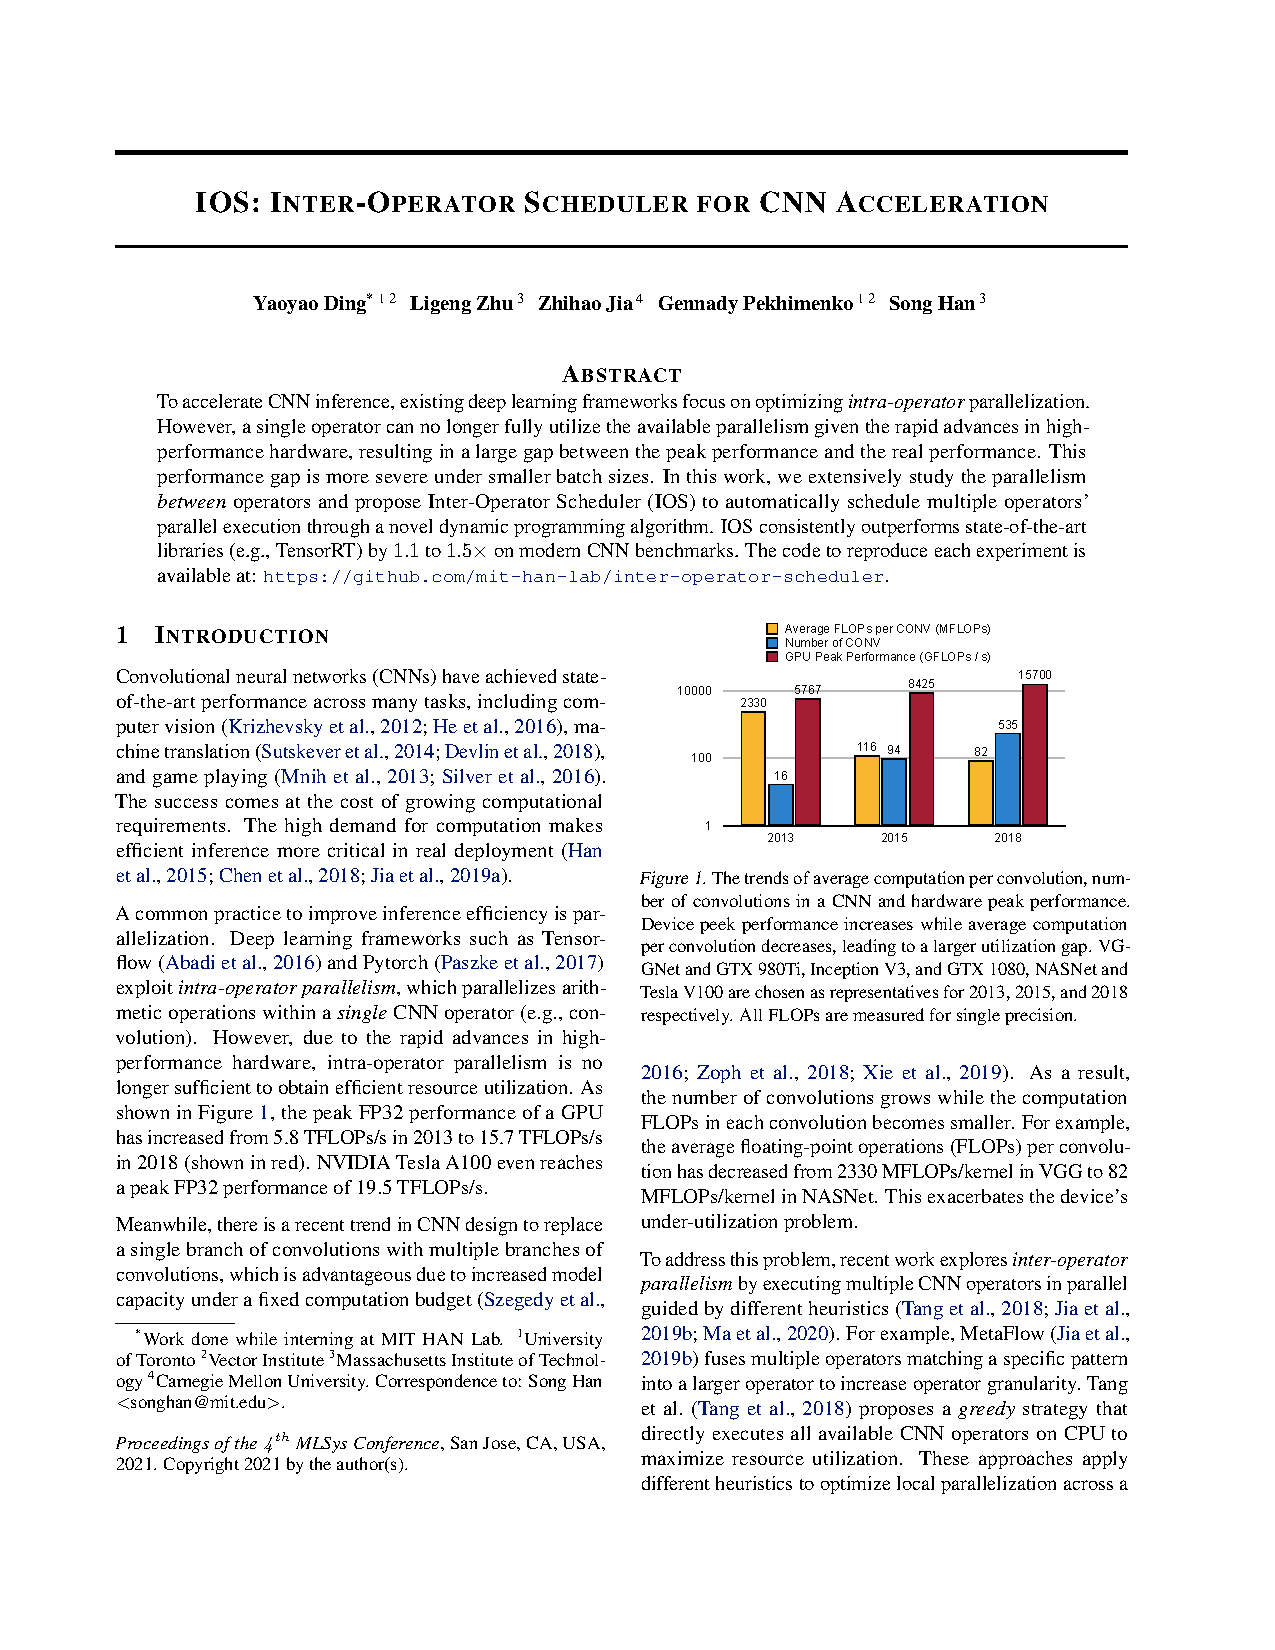
\includegraphics[page=1,trim=11.5cm 13.5cm 3.5cm 10.2cm,clip,scale=1]{paper.pdf}
            \end{column}
        \end{columns}
    \end{frame}

    \begin{frame}
        \frametitle{Existing Approaches}

        \begin{itemize}
            \setlength{\itemsep}{.8em}
            \item \textbf{Intra-operator parallelism} (TVM) executes arithmetic operations within a single operator in
                  parallel. However, the degree of parallelism within an operator is limited, especially when the
                  \texttt{Conv} operations are becoming smaller.
            \item \textbf{Graph transformation} (MetaFlow, TASO) explores merging and substituting operators to enable
                  more parallelism. However, the possible merging are limited to same type of operators.
            \item \textbf{Inter-operator scheduling} (Graphi, Rammer, Nimble) schedules some operators to run
                  concurrently. However, they use simple heuristics and don't lead to global optimal.
        \end{itemize}
    \end{frame}

    \begin{frame}
        \frametitle{IOS: Inter-Operator Scheduler}

        This paper introduces \textbf{IOS}, a novel \textbf{dynamic programming} algorithm to find a highly optimized schedule
        for \textbf{inter-operator parallelization}.
    \end{frame}

    \section{Problem Definition}

    \begin{frame}
        \frametitle{Graph and Stage}

        \begin{columns}
            \begin{column}{0.5\textwidth}
                A CNN is defined as a DAG $G = (V, E)$, where $V$ is the set of operators, and $E$ is the edge set
                representing dependencies.
                \vskip 1em

                The computation graph is partitioned into multiple \textbf{stages}. Stages are executed sequentially and
                the operators in the same stage are executed according to a certain \textbf{parallelization strategy}.
            \end{column}
            \begin{column}{0.5\textwidth}
                \includegraphics[page=4,trim=2.2cm 20cm 11.5cm 2.2cm,clip,scale=0.88]{paper.pdf}
            \end{column}
        \end{columns}
    \end{frame}

    \begin{frame}
        \frametitle{Parallelization Strategy}

        \begin{columns}
            \begin{column}{0.5\textwidth}
                \textbf{Operator merge} merges multiple operators of the \textbf{same type} together. For example, an
                3x3 \texttt{Conv} can be merged with a 5x5 \texttt{Conv}, by padding and concatenating the kernels.
                \vskip 1em

                Under \textbf{concurrent execution}, the operators in the stage that have no dependencies are executed
                concurrently with multiple CUDA streams.
            \end{column}
            \begin{column}{0.5\textwidth}
                \includegraphics[page=4,trim=2.2cm 20cm 11.5cm 2.2cm,clip,scale=0.88]{paper.pdf}
            \end{column}
        \end{columns}
    \end{frame}

    \begin{frame}
        \frametitle{Schedule}

        \begin{columns}
            \begin{column}{0.5\textwidth}
                A Schedule $Q = \{(S_1, T_1), (S_2, T_2), \dots\}$ is an assignment of operators $S_i$ to the i-th stage
                and the parallelization strategy $T_i$ of the i-th stage.
                \vskip 1em

                IOS finds a schedule $Q^*$ that minimizes a cost function $c$ for a given graph $G$, i.e.,
                $Q^* = \text{argmin}_Qc(G,Q)$. In this work, $c$ is defined as the latency of running $G$ following
                schedule $Q$.
            \end{column}
            \begin{column}{0.5\textwidth}
                \includegraphics[page=4,trim=2.2cm 20cm 11.5cm 2.2cm,clip,scale=0.88]{paper.pdf}
            \end{column}
        \end{columns}
    \end{frame}

    \section{Methods}

    \begin{frame}
        \frametitle{Main Idea}

        For an \textbf{ending} $S'$ of $S$, we have:

        $$ \text{cost}[S] = \min_{S'}(\text{cost}[S - S'] + \text{stage\_latency}[S']) $$

        \vskip 1em
        \centering
        \includegraphics[page=4,trim=10.5cm 8.2cm 2.2cm 16.6cm,clip,scale=1]{paper.pdf}
    \end{frame}

    \begin{frame}
        \frametitle{Core Function}

        \centering
        \includegraphics[page=5,trim=11.3cm 15.9cm 2.2cm 8.2cm,clip,scale=1]{paper.pdf}
    \end{frame}

    \begin{frame}
        \frametitle{Example}

        \vskip -2em
        \centering
        \includegraphics[page=6,trim=1.5cm 13.3cm 2.4cm 2.2cm,clip,scale=0.65]{paper.pdf}
    \end{frame}

    \begin{frame}
        \frametitle{Time Complexity}

        \textbf{Definition}: $d$ is the width of $G$, if we can find at most $d$ operators in $G$ such that there is no
        path connecting any two of them.

        \vskip 1em
        \textbf{Theorem}: The time complexity of IOS is $\mathcal{O}({n/d+2 \choose 2}^d)$, which can be
        relaxed to $\mathcal{O}((n/d+1)^{2d})$, where $n$ is the number of operators in $G$ and $d$ is its width.

        \vskip 1em
        \centering
        \includegraphics[page=7,trim=2.2cm 18cm 11.5cm 7.5cm,clip,scale=1]{paper.pdf}
    \end{frame}

    \begin{frame}
        \frametitle{Pruning}

        IOS without pruning can find the optimal strategy for the benchmarked graphs in 4 hours. To further reduce the
        search time, IOS introduces two parameters $r$ and $s$. $P_{r,s}(S, S') = \text{True}$ if and only if $S'$ has at most
        $s$ groups and each group has at most $r$ operators.
    \end{frame}

    \section{Evaluation}

    \begin{frame}
        \frametitle{Experiments Setup}

        \begin{itemize}
            \setlength{\itemsep}{.8em}
            \item Hardware: NVIDIA Tesla V100
            \item Execution Engine: A cuDNN-based C++ execution engine.
            \item Models: Inception V3, RandWire, NasNet-A, and SqueezeNet
            \item Baselines: TensorRT and TVM
            \item Pruning Parameters: $r = 3$ and $s = 8$
        \end{itemize}
    \end{frame}

    \begin{frame}
        \frametitle{Comparison of Different Schedules}

        \begin{center}
            \includegraphics[page=8,trim=1.8cm 22.2cm 11cm 2.2cm,clip,scale=1.2]{paper.pdf}
        \end{center}
    \end{frame}

    \begin{frame}
        \frametitle{Comparison of cuDNN-based Frameworks}

        \begin{center}
            \includegraphics[page=8,trim=10.6cm 22.2cm 2.2cm 2.2cm,clip,scale=1.2]{paper.pdf}
        \end{center}
    \end{frame}

    \begin{frame}
        \frametitle{More Active Warps Improve Utilization}

        \begin{center}
            \includegraphics[page=8,trim=10.6cm 7.7cm 2.2cm 17cm,clip,scale=1.2]{paper.pdf}
        \end{center}
    \end{frame}

    \begin{frame}
        \frametitle{Schedule Pruning Reduces Search Time}

        \begin{center}
            \includegraphics[page=9,trim=1.8cm 10.7cm 11cm 11.2cm,clip,scale=1]{paper.pdf}
        \end{center}
    \end{frame}

    \begin{frame}
        \frametitle{Specialized Scheduling is Beneficial}

        \begin{center}
            \includegraphics[page=9,trim=10.6cm 22.1cm 2.2cm 3cm,clip,scale=1.2]{paper.pdf}
        \end{center}
    \end{frame}

    \begin{frame}
        \frametitle{Consistent Improvement for Different Batch Sizes}

        \begin{center}
            \includegraphics[page=10,trim=1.8cm 10.7cm 11cm 13.2cm,clip,scale=1.1]{paper.pdf}
        \end{center}
    \end{frame}

    \begin{frame}
        \frametitle{Intra- and Inter-Operator Parallelism}

        \begin{center}
            \includegraphics[page=10,trim=10.6cm 21.9cm 2.2cm 3cm,clip,scale=1.1]{paper.pdf}
        \end{center}
    \end{frame}

    \section{Summary}

    \begin{frame}
        \frametitle{Conclusion}

        \textbf{Strength}

        \vskip .6em
        \begin{itemize}
            \setlength{\itemsep}{.8em}
            \item IOS introduces the concept of \textbf{stage}, which enables dynamic programming.
            \item The algorithm description is detailed and the open-sourced code is clean.
        \end{itemize}

        \vskip 1em
        \textbf{Limitation}

        \vskip .6em
        \begin{itemize}
            \setlength{\itemsep}{.8em}
            \item The paper omits the detail about the profiler. IOS needs the cost of running multiple operators
                  concurrently, which is not easy to simulate.
            \item The strategy space is very limited (compared with related works).
            \item They do not compare with similar works (Rammer etc.) in experiments.
        \end{itemize}
    \end{frame}

    \begin{frame}
        \frametitle{Takeaways}

        \begin{itemize}
            \setlength{\itemsep}{.8em}
            \item Dynamic programming works well with the DAG structure of neural networks. Other works have explored
                  using dynamic programming for saving memory, distributed training, etc.
            \item We can design a reduced search space and use an efficient algorithm to find the global optimal.
        \end{itemize}
    \end{frame}

    \appendix

    \begin{frame}
        \vskip 1.5em

        \centering \huge
        Thank you!
    \end{frame}
\end{document}
